%!TEX root = ./intern_report.tex

\newpage
\subsection{Life at CSIRO}

\paragraph{}
CSIRO, being a world class research institute, thrives to create a stress-free work environment that encourages people to socialize and to boost creativity. There is a workplace culture in DATA61 to bring cakes (or any equivalent sweets) for all the coworkers if one gets married, arrive at CSIRO, leave CSIRO, has a birthday and so on. I shared Sri Lankan sweets (sent by my mother in mail) for my birthday and cakes with everyone for arriving at and leaving CSIRO.

\subsubsection{Reading Groups and DATA61 Meetings}

\paragraph{}
Every friday, a small meeting called "Robotics Reading Group" is hosted, where one scientist explains his current project to everyone who attends the meeting. This way, we get to know the latest technology that is being developed in different parts of DATA61 and new projects that are being started. This meeting also allows the scientist to be questioned, so that he can derive insights from the audience and refine his procedures in the future. Also, once in a fortnight our supervisor Nick holds a "ML Robotics" meeting for all engineers working on machine learning. There we discuss our current ideas and issues to help each other. In addition to these, there are monthly meetings with the entire CSIRO (branches from all over Australia join via video conferencing), where new developments are discussed. One such meeting had the lead scientist from NASA's Insight Mars Lander mission as the chief guest explaining the challenges faced in their mission and taking our questions on the matter.

\begin{figure}[H]
    \centering
    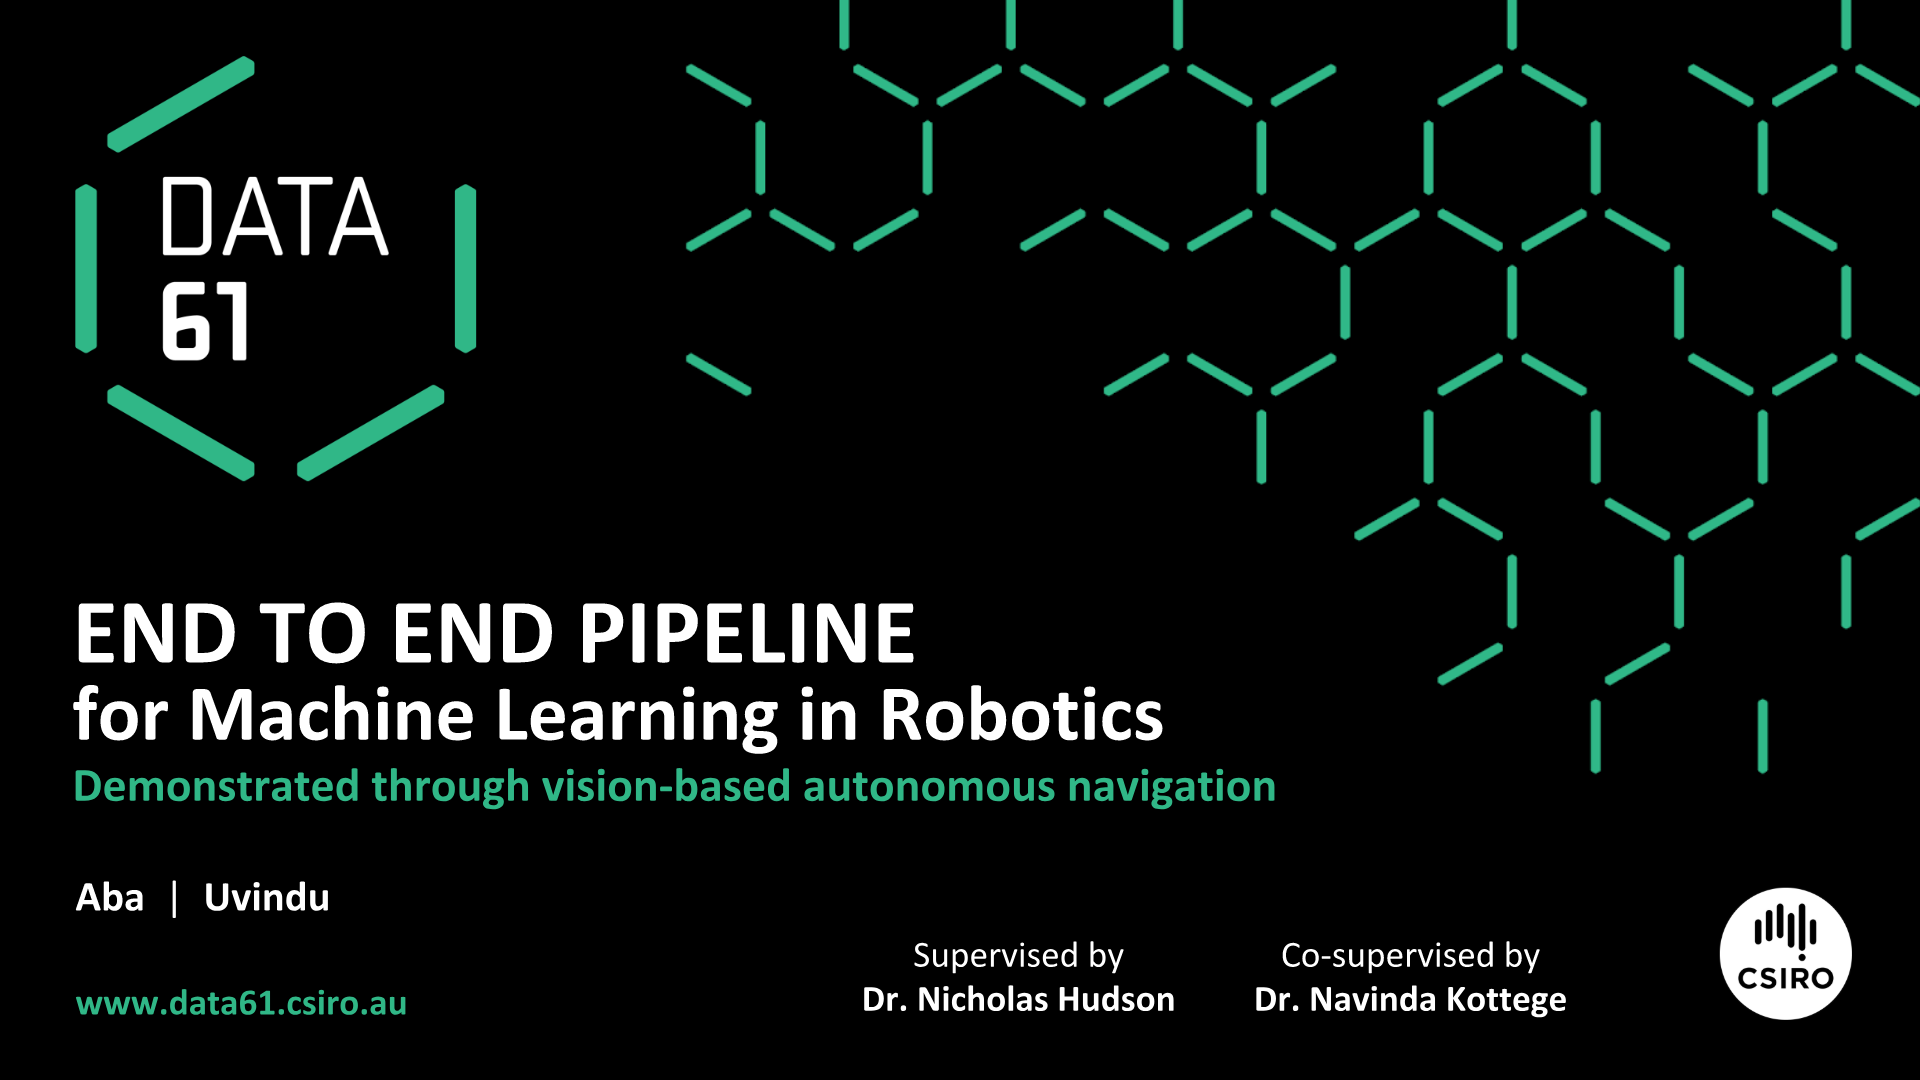
\includegraphics
        [width=12cm]
        {figures/presentation.png}
    \caption{Presenting the Pipeline in Robotics Reading Group}\vspace{-4mm}
\end{figure}

\subsubsection{Presenting the Pipeline at Reading Group to the Scientists}

Uvindu and I presented the pipeline to other scientists during one of the last Reading Group meetings of the year. It was well received, thanks to the support of our supervisor who encouraged others to use our pipeline in their workflow. Many asked questions and were convinced of the merits of such a unified framework. I had a few scientists reaching out to me on the following days asking me to develop visualization tools to complement the pipeline. 

\subsubsection{DATA61 Live Event}

DATA61 Live is an event held annually to showcase the science and technology innovations of DATA61 from all over Australia. In 2018, it was held in Brisbane, in our city. The theme was: 'Adapting to Disruption'. We signed up as volunteers and apart from volunteering, we had a chance to attend many lectures, talks and forums. It was a great experience.

\begin{figure}[H]
    \centering
    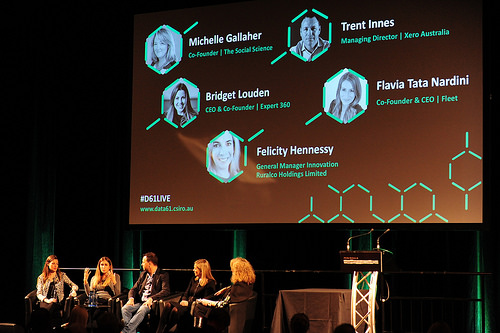
\includegraphics
        [height=5cm]
        {figures/data61_live_1.jpg}
    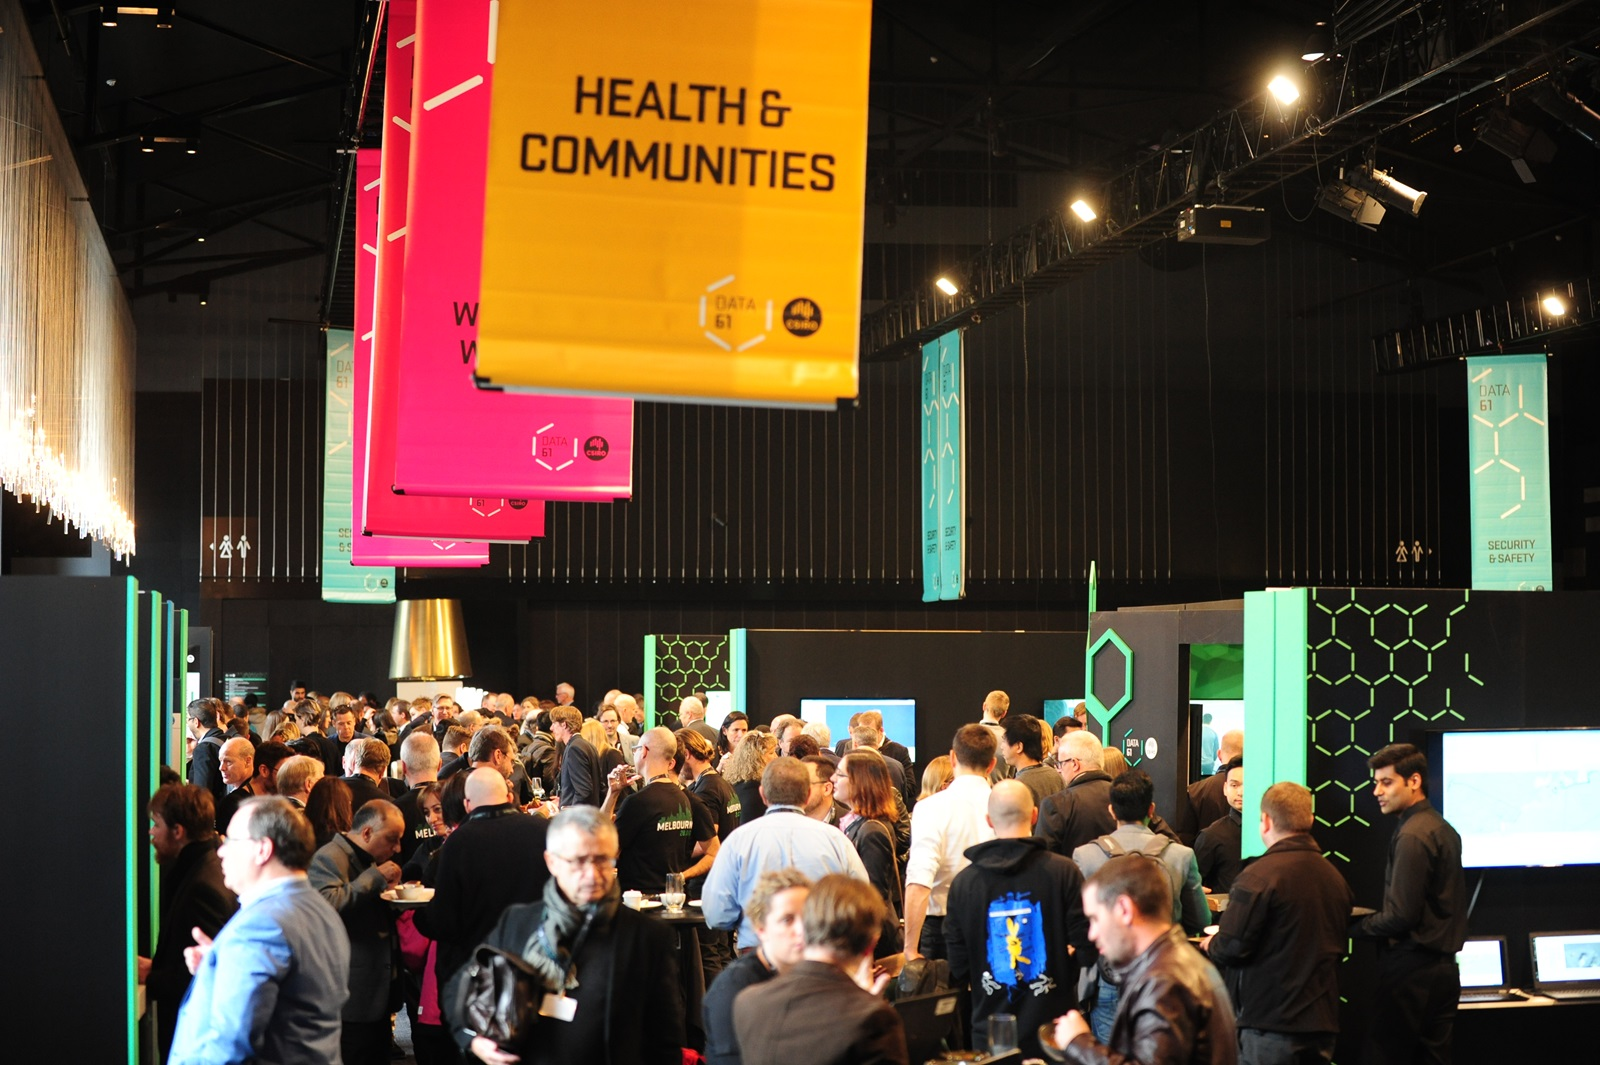
\includegraphics
        [height=5cm]
        {figures/data61_live_2.jpg}
    \caption{DATA61 LIVE Event}\vspace{-4mm}
\end{figure}